% Options for packages loaded elsewhere
\PassOptionsToPackage{unicode}{hyperref}
\PassOptionsToPackage{hyphens}{url}
%
\documentclass[
]{article}
\usepackage{amsmath,amssymb}
\usepackage{lmodern}
\usepackage{iftex}
\ifPDFTeX
  \usepackage[T1]{fontenc}
  \usepackage[utf8]{inputenc}
  \usepackage{textcomp} % provide euro and other symbols
\else % if luatex or xetex
  \usepackage{unicode-math}
  \defaultfontfeatures{Scale=MatchLowercase}
  \defaultfontfeatures[\rmfamily]{Ligatures=TeX,Scale=1}
\fi
% Use upquote if available, for straight quotes in verbatim environments
\IfFileExists{upquote.sty}{\usepackage{upquote}}{}
\IfFileExists{microtype.sty}{% use microtype if available
  \usepackage[]{microtype}
  \UseMicrotypeSet[protrusion]{basicmath} % disable protrusion for tt fonts
}{}
\makeatletter
\@ifundefined{KOMAClassName}{% if non-KOMA class
  \IfFileExists{parskip.sty}{%
    \usepackage{parskip}
  }{% else
    \setlength{\parindent}{0pt}
    \setlength{\parskip}{6pt plus 2pt minus 1pt}}
}{% if KOMA class
  \KOMAoptions{parskip=half}}
\makeatother
\usepackage{xcolor}
\IfFileExists{xurl.sty}{\usepackage{xurl}}{} % add URL line breaks if available
\IfFileExists{bookmark.sty}{\usepackage{bookmark}}{\usepackage{hyperref}}
\hypersetup{
  pdftitle={Modelo Logit},
  pdfauthor={David Arango  Daniel Gonzalez},
  hidelinks,
  pdfcreator={LaTeX via pandoc}}
\urlstyle{same} % disable monospaced font for URLs
\usepackage[margin=1in]{geometry}
\usepackage{color}
\usepackage{fancyvrb}
\newcommand{\VerbBar}{|}
\newcommand{\VERB}{\Verb[commandchars=\\\{\}]}
\DefineVerbatimEnvironment{Highlighting}{Verbatim}{commandchars=\\\{\}}
% Add ',fontsize=\small' for more characters per line
\usepackage{framed}
\definecolor{shadecolor}{RGB}{248,248,248}
\newenvironment{Shaded}{\begin{snugshade}}{\end{snugshade}}
\newcommand{\AlertTok}[1]{\textcolor[rgb]{0.94,0.16,0.16}{#1}}
\newcommand{\AnnotationTok}[1]{\textcolor[rgb]{0.56,0.35,0.01}{\textbf{\textit{#1}}}}
\newcommand{\AttributeTok}[1]{\textcolor[rgb]{0.77,0.63,0.00}{#1}}
\newcommand{\BaseNTok}[1]{\textcolor[rgb]{0.00,0.00,0.81}{#1}}
\newcommand{\BuiltInTok}[1]{#1}
\newcommand{\CharTok}[1]{\textcolor[rgb]{0.31,0.60,0.02}{#1}}
\newcommand{\CommentTok}[1]{\textcolor[rgb]{0.56,0.35,0.01}{\textit{#1}}}
\newcommand{\CommentVarTok}[1]{\textcolor[rgb]{0.56,0.35,0.01}{\textbf{\textit{#1}}}}
\newcommand{\ConstantTok}[1]{\textcolor[rgb]{0.00,0.00,0.00}{#1}}
\newcommand{\ControlFlowTok}[1]{\textcolor[rgb]{0.13,0.29,0.53}{\textbf{#1}}}
\newcommand{\DataTypeTok}[1]{\textcolor[rgb]{0.13,0.29,0.53}{#1}}
\newcommand{\DecValTok}[1]{\textcolor[rgb]{0.00,0.00,0.81}{#1}}
\newcommand{\DocumentationTok}[1]{\textcolor[rgb]{0.56,0.35,0.01}{\textbf{\textit{#1}}}}
\newcommand{\ErrorTok}[1]{\textcolor[rgb]{0.64,0.00,0.00}{\textbf{#1}}}
\newcommand{\ExtensionTok}[1]{#1}
\newcommand{\FloatTok}[1]{\textcolor[rgb]{0.00,0.00,0.81}{#1}}
\newcommand{\FunctionTok}[1]{\textcolor[rgb]{0.00,0.00,0.00}{#1}}
\newcommand{\ImportTok}[1]{#1}
\newcommand{\InformationTok}[1]{\textcolor[rgb]{0.56,0.35,0.01}{\textbf{\textit{#1}}}}
\newcommand{\KeywordTok}[1]{\textcolor[rgb]{0.13,0.29,0.53}{\textbf{#1}}}
\newcommand{\NormalTok}[1]{#1}
\newcommand{\OperatorTok}[1]{\textcolor[rgb]{0.81,0.36,0.00}{\textbf{#1}}}
\newcommand{\OtherTok}[1]{\textcolor[rgb]{0.56,0.35,0.01}{#1}}
\newcommand{\PreprocessorTok}[1]{\textcolor[rgb]{0.56,0.35,0.01}{\textit{#1}}}
\newcommand{\RegionMarkerTok}[1]{#1}
\newcommand{\SpecialCharTok}[1]{\textcolor[rgb]{0.00,0.00,0.00}{#1}}
\newcommand{\SpecialStringTok}[1]{\textcolor[rgb]{0.31,0.60,0.02}{#1}}
\newcommand{\StringTok}[1]{\textcolor[rgb]{0.31,0.60,0.02}{#1}}
\newcommand{\VariableTok}[1]{\textcolor[rgb]{0.00,0.00,0.00}{#1}}
\newcommand{\VerbatimStringTok}[1]{\textcolor[rgb]{0.31,0.60,0.02}{#1}}
\newcommand{\WarningTok}[1]{\textcolor[rgb]{0.56,0.35,0.01}{\textbf{\textit{#1}}}}
\usepackage{graphicx}
\makeatletter
\def\maxwidth{\ifdim\Gin@nat@width>\linewidth\linewidth\else\Gin@nat@width\fi}
\def\maxheight{\ifdim\Gin@nat@height>\textheight\textheight\else\Gin@nat@height\fi}
\makeatother
% Scale images if necessary, so that they will not overflow the page
% margins by default, and it is still possible to overwrite the defaults
% using explicit options in \includegraphics[width, height, ...]{}
\setkeys{Gin}{width=\maxwidth,height=\maxheight,keepaspectratio}
% Set default figure placement to htbp
\makeatletter
\def\fps@figure{htbp}
\makeatother
\setlength{\emergencystretch}{3em} % prevent overfull lines
\providecommand{\tightlist}{%
  \setlength{\itemsep}{0pt}\setlength{\parskip}{0pt}}
\setcounter{secnumdepth}{-\maxdimen} % remove section numbering
\ifLuaTeX
  \usepackage{selnolig}  % disable illegal ligatures
\fi

\title{\textbf{Modelo Logit}}
\usepackage{etoolbox}
\makeatletter
\providecommand{\subtitle}[1]{% add subtitle to \maketitle
  \apptocmd{\@title}{\par {\large #1 \par}}{}{}
}
\makeatother
\subtitle{{\textbf{Unidad 1}}}
\author{David Arango Daniel Gonzalez}
\date{}

\begin{document}
\maketitle

{
\setcounter{tocdepth}{2}
\tableofcontents
}
\hypertarget{problema}{%
\section{Problema}\label{problema}}

El siguiente problema es tomado del documento realizado por
\href{https://rpubs.com/Joaquin_AR/229736}{Joaquín Amat Rodrigo}
publicado en RPlus con el fin de presentar el modelo logit simple

\hypertarget{objetivo}{%
\subsection{Objetivo}\label{objetivo}}

\begin{itemize}
\item
  Ilustrar los componentes del modelo lineal general para el caso
  particular del modelo de logit simple, enmarcado dentro de los modelos
  llamados \textbf{modelos de probabilidad}
\item
  Determinar la probabilidad de que un estudiante obtenga matricula de
  honor a partir de la nota obtenida en matemáticas
\end{itemize}

\hypertarget{preguntas-que-surgen}{%
\subsection{Preguntas que surgen}\label{preguntas-que-surgen}}

\begin{itemize}
\tightlist
\item
  Cómo se estiman los modelos de regresión con variables cualitativas
  como variables respuesta?
\item
  Qué problemas se presentan cuando se desean realizar inferencias? Que
  pruebas de hipotesis se deben realizar?
\item
  Como se mide la bondad de ajuste del modelo estimado?
\item
  Como se interpretan los resultados obtenidos?
\end{itemize}

Preguntas planteadas en Gujarati(2009)

Con el prósito de responder a esta preguntas, empezaremos con las
caracteristicas de los datos

\hypertarget{datos}{%
\subsection{Datos}\label{datos}}

La siguiente data contiene los datos de un conjunto de estudiantes que
han obtenido matreicua de honor (matricula =1) y un grupo de no la han
conseguido (matricula =0) y sus respectivas notas obtenidas en
matemáticas

En este caso se debe contar con una variable categótica con dos niveles
representados por dos valores : 0 y 1 (variable matricula), quien obra
como variable dependiente y por lo menos una variable cuantitativa que
tome diferentes valores (en este caso la nota de matemáticas).

\begin{Shaded}
\begin{Highlighting}[]
\NormalTok{matricula }\OtherTok{\textless{}{-}} \FunctionTok{c}\NormalTok{(}\DecValTok{0}\NormalTok{, }\DecValTok{0}\NormalTok{, }\DecValTok{0}\NormalTok{, }\DecValTok{0}\NormalTok{, }\DecValTok{0}\NormalTok{, }\DecValTok{0}\NormalTok{, }\DecValTok{0}\NormalTok{, }\DecValTok{0}\NormalTok{, }\DecValTok{0}\NormalTok{, }\DecValTok{0}\NormalTok{, }\DecValTok{0}\NormalTok{, }\DecValTok{1}\NormalTok{, }\DecValTok{0}\NormalTok{, }\DecValTok{1}\NormalTok{, }\DecValTok{0}\NormalTok{, }\DecValTok{0}\NormalTok{, }\DecValTok{0}\NormalTok{, }\DecValTok{0}\NormalTok{, }\DecValTok{1}\NormalTok{, }\DecValTok{0}\NormalTok{, }\DecValTok{0}\NormalTok{, }\DecValTok{1}\NormalTok{, }\DecValTok{0}\NormalTok{, }\DecValTok{0}\NormalTok{, }\DecValTok{0}\NormalTok{, }\DecValTok{0}\NormalTok{, }\DecValTok{1}\NormalTok{, }\DecValTok{0}\NormalTok{, }\DecValTok{0}\NormalTok{, }\DecValTok{0}\NormalTok{, }\DecValTok{0}\NormalTok{, }\DecValTok{0}\NormalTok{, }\DecValTok{1}\NormalTok{, }\DecValTok{0}\NormalTok{, }\DecValTok{0}\NormalTok{, }\DecValTok{1}\NormalTok{, }\DecValTok{0}\NormalTok{, }\DecValTok{1}\NormalTok{, }\DecValTok{0}\NormalTok{, }\DecValTok{0}\NormalTok{, }\DecValTok{0}\NormalTok{, }\DecValTok{0}\NormalTok{, }\DecValTok{0}\NormalTok{, }\DecValTok{0}\NormalTok{, }\DecValTok{1}\NormalTok{, }\DecValTok{0}\NormalTok{, }\DecValTok{0}\NormalTok{, }\DecValTok{0}\NormalTok{, }\DecValTok{0}\NormalTok{, }\DecValTok{0}\NormalTok{, }\DecValTok{1}\NormalTok{, }\DecValTok{0}\NormalTok{, }\DecValTok{0}\NormalTok{, }\DecValTok{0}\NormalTok{, }\DecValTok{1}\NormalTok{, }\DecValTok{0}\NormalTok{, }\DecValTok{0}\NormalTok{, }\DecValTok{0}\NormalTok{, }\DecValTok{0}\NormalTok{, }\DecValTok{0}\NormalTok{, }\DecValTok{0}\NormalTok{, }\DecValTok{1}\NormalTok{, }\DecValTok{0}\NormalTok{, }\DecValTok{0}\NormalTok{, }\DecValTok{0}\NormalTok{, }\DecValTok{0}\NormalTok{, }\DecValTok{0}\NormalTok{, }\DecValTok{0}\NormalTok{, }\DecValTok{0}\NormalTok{, }\DecValTok{0}\NormalTok{, }\DecValTok{0}\NormalTok{, }\DecValTok{0}\NormalTok{, }\DecValTok{1}\NormalTok{, }\DecValTok{0}\NormalTok{, }\DecValTok{0}\NormalTok{, }\DecValTok{0}\NormalTok{, }\DecValTok{1}\NormalTok{, }\DecValTok{0}\NormalTok{, }\DecValTok{0}\NormalTok{, }\DecValTok{0}\NormalTok{, }\DecValTok{0}\NormalTok{, }\DecValTok{0}\NormalTok{, }\DecValTok{0}\NormalTok{, }\DecValTok{1}\NormalTok{, }\DecValTok{0}\NormalTok{, }\DecValTok{1}\NormalTok{, }\DecValTok{0}\NormalTok{, }\DecValTok{0}\NormalTok{, }\DecValTok{0}\NormalTok{, }\DecValTok{0}\NormalTok{, }\DecValTok{1}\NormalTok{, }\DecValTok{0}\NormalTok{, }\DecValTok{1}\NormalTok{, }\DecValTok{0}\NormalTok{, }\DecValTok{0}\NormalTok{, }\DecValTok{1}\NormalTok{, }\DecValTok{1}\NormalTok{, }\DecValTok{1}\NormalTok{, }\DecValTok{0}\NormalTok{, }\DecValTok{1}\NormalTok{, }\DecValTok{0}\NormalTok{, }\DecValTok{0}\NormalTok{, }\DecValTok{0}\NormalTok{, }\DecValTok{0}\NormalTok{, }\DecValTok{0}\NormalTok{, }\DecValTok{0}\NormalTok{, }\DecValTok{1}\NormalTok{, }\DecValTok{0}\NormalTok{, }\DecValTok{0}\NormalTok{, }\DecValTok{1}\NormalTok{, }\DecValTok{0}\NormalTok{, }\DecValTok{0}\NormalTok{, }\DecValTok{0}\NormalTok{, }\DecValTok{1}\NormalTok{,  }\DecValTok{1}\NormalTok{, }\DecValTok{0}\NormalTok{, }\DecValTok{0}\NormalTok{, }\DecValTok{1}\NormalTok{, }\DecValTok{0}\NormalTok{, }\DecValTok{0}\NormalTok{, }\DecValTok{0}\NormalTok{, }\DecValTok{0}\NormalTok{, }\DecValTok{0}\NormalTok{, }\DecValTok{0}\NormalTok{, }\DecValTok{1}\NormalTok{, }\DecValTok{0}\NormalTok{, }\DecValTok{0}\NormalTok{, }\DecValTok{0}\NormalTok{, }\DecValTok{0}\NormalTok{, }\DecValTok{0}\NormalTok{, }\DecValTok{0}\NormalTok{, }\DecValTok{1}\NormalTok{, }\DecValTok{1}\NormalTok{, }\DecValTok{0}\NormalTok{, }\DecValTok{0}\NormalTok{, }\DecValTok{1}\NormalTok{, }\DecValTok{0}\NormalTok{, }\DecValTok{0}\NormalTok{, }\DecValTok{0}\NormalTok{, }\DecValTok{0}\NormalTok{, }\DecValTok{0}\NormalTok{, }\DecValTok{0}\NormalTok{, }\DecValTok{0}\NormalTok{, }\DecValTok{0}\NormalTok{, }\DecValTok{0}\NormalTok{, }\DecValTok{0}\NormalTok{, }\DecValTok{1}\NormalTok{, }\DecValTok{0}\NormalTok{, }\DecValTok{0}\NormalTok{, }\DecValTok{0}\NormalTok{, }\DecValTok{0}\NormalTok{, }\DecValTok{0}\NormalTok{, }\DecValTok{0}\NormalTok{, }\DecValTok{0}\NormalTok{, }\DecValTok{1}\NormalTok{, }\DecValTok{0}\NormalTok{, }\DecValTok{0}\NormalTok{, }\DecValTok{0}\NormalTok{, }\DecValTok{0}\NormalTok{, }\DecValTok{1}\NormalTok{, }\DecValTok{1}\NormalTok{, }\DecValTok{0}\NormalTok{, }\DecValTok{1}\NormalTok{, }\DecValTok{1}\NormalTok{, }\DecValTok{0}\NormalTok{, }\DecValTok{0}\NormalTok{, }\DecValTok{0}\NormalTok{, }\DecValTok{0}\NormalTok{, }\DecValTok{1}\NormalTok{, }\DecValTok{0}\NormalTok{, }\DecValTok{0}\NormalTok{, }\DecValTok{0}\NormalTok{, }\DecValTok{0}\NormalTok{, }\DecValTok{0}\NormalTok{, }\DecValTok{0}\NormalTok{, }\DecValTok{0}\NormalTok{, }\DecValTok{1}\NormalTok{, }\DecValTok{0}\NormalTok{, }\DecValTok{0}\NormalTok{, }\DecValTok{1}\NormalTok{, }\DecValTok{1}\NormalTok{, }\DecValTok{0}\NormalTok{, }\DecValTok{1}\NormalTok{, }\DecValTok{1}\NormalTok{, }\DecValTok{1}\NormalTok{, }\DecValTok{1}\NormalTok{, }\DecValTok{0}\NormalTok{, }\DecValTok{0}\NormalTok{, }\DecValTok{1}\NormalTok{, }\DecValTok{0}\NormalTok{, }\DecValTok{0}\NormalTok{, }\DecValTok{0}\NormalTok{, }\DecValTok{0}\NormalTok{, }\DecValTok{0}\NormalTok{, }\DecValTok{1}\NormalTok{, }\DecValTok{0}\NormalTok{, }\DecValTok{0}\NormalTok{, }\DecValTok{0}\NormalTok{, }\DecValTok{1}\NormalTok{, }\DecValTok{1}\NormalTok{)}
\NormalTok{matematicas }\OtherTok{\textless{}{-}} \FunctionTok{c}\NormalTok{(}\DecValTok{41}\NormalTok{, }\DecValTok{53}\NormalTok{, }\DecValTok{54}\NormalTok{, }\DecValTok{47}\NormalTok{, }\DecValTok{57}\NormalTok{, }\DecValTok{51}\NormalTok{, }\DecValTok{42}\NormalTok{, }\DecValTok{45}\NormalTok{, }\DecValTok{54}\NormalTok{, }\DecValTok{52}\NormalTok{, }\DecValTok{51}\NormalTok{, }\DecValTok{51}\NormalTok{, }\DecValTok{71}\NormalTok{, }\DecValTok{57}\NormalTok{, }\DecValTok{50}\NormalTok{, }\DecValTok{43}\NormalTok{, }\DecValTok{51}\NormalTok{, }\DecValTok{60}\NormalTok{, }\DecValTok{62}\NormalTok{, }\DecValTok{57}\NormalTok{, }\DecValTok{35}\NormalTok{, }\DecValTok{75}\NormalTok{, }\DecValTok{45}\NormalTok{, }\DecValTok{57}\NormalTok{, }\DecValTok{45}\NormalTok{, }\DecValTok{46}\NormalTok{, }\DecValTok{66}\NormalTok{, }\DecValTok{57}\NormalTok{, }\DecValTok{49}\NormalTok{, }\DecValTok{49}\NormalTok{, }\DecValTok{57}\NormalTok{, }\DecValTok{64}\NormalTok{, }\DecValTok{63}\NormalTok{, }\DecValTok{57}\NormalTok{, }\DecValTok{50}\NormalTok{, }\DecValTok{58}\NormalTok{, }\DecValTok{75}\NormalTok{, }\DecValTok{68}\NormalTok{, }\DecValTok{44}\NormalTok{, }\DecValTok{40}\NormalTok{, }\DecValTok{41}\NormalTok{, }\DecValTok{62}\NormalTok{, }\DecValTok{57}\NormalTok{, }\DecValTok{43}\NormalTok{, }\DecValTok{48}\NormalTok{, }\DecValTok{63}\NormalTok{, }\DecValTok{39}\NormalTok{, }\DecValTok{70}\NormalTok{, }\DecValTok{63}\NormalTok{, }\DecValTok{59}\NormalTok{, }\DecValTok{61}\NormalTok{, }\DecValTok{38}\NormalTok{, }\DecValTok{61}\NormalTok{, }\DecValTok{49}\NormalTok{, }\DecValTok{73}\NormalTok{, }\DecValTok{44}\NormalTok{, }\DecValTok{42}\NormalTok{, }\DecValTok{39}\NormalTok{, }\DecValTok{55}\NormalTok{, }\DecValTok{52}\NormalTok{, }\DecValTok{45}\NormalTok{, }\DecValTok{61}\NormalTok{, }\DecValTok{39}\NormalTok{, }\DecValTok{41}\NormalTok{, }\DecValTok{50}\NormalTok{, }\DecValTok{40}\NormalTok{, }\DecValTok{60}\NormalTok{, }\DecValTok{47}\NormalTok{, }\DecValTok{59}\NormalTok{, }\DecValTok{49}\NormalTok{, }\DecValTok{46}\NormalTok{, }\DecValTok{58}\NormalTok{, }\DecValTok{71}\NormalTok{, }\DecValTok{58}\NormalTok{, }\DecValTok{46}\NormalTok{, }\DecValTok{43}\NormalTok{, }\DecValTok{54}\NormalTok{, }\DecValTok{56}\NormalTok{, }\DecValTok{46}\NormalTok{, }\DecValTok{54}\NormalTok{, }\DecValTok{57}\NormalTok{, }\DecValTok{54}\NormalTok{, }\DecValTok{71}\NormalTok{, }\DecValTok{48}\NormalTok{, }\DecValTok{40}\NormalTok{, }\DecValTok{64}\NormalTok{, }\DecValTok{51}\NormalTok{, }\DecValTok{39}\NormalTok{, }\DecValTok{40}\NormalTok{, }\DecValTok{61}\NormalTok{, }\DecValTok{66}\NormalTok{, }\DecValTok{49}\NormalTok{, }\DecValTok{65}\NormalTok{, }\DecValTok{52}\NormalTok{, }\DecValTok{46}\NormalTok{, }\DecValTok{61}\NormalTok{, }\DecValTok{72}\NormalTok{, }\DecValTok{71}\NormalTok{, }\DecValTok{40}\NormalTok{, }\DecValTok{69}\NormalTok{, }\DecValTok{64}\NormalTok{, }\DecValTok{56}\NormalTok{, }\DecValTok{49}\NormalTok{, }\DecValTok{54}\NormalTok{, }\DecValTok{53}\NormalTok{, }\DecValTok{66}\NormalTok{, }\DecValTok{67}\NormalTok{, }\DecValTok{40}\NormalTok{, }\DecValTok{46}\NormalTok{, }\DecValTok{69}\NormalTok{, }\DecValTok{40}\NormalTok{, }\DecValTok{41}\NormalTok{, }\DecValTok{57}\NormalTok{, }\DecValTok{58}\NormalTok{, }\DecValTok{57}\NormalTok{, }\DecValTok{37}\NormalTok{, }\DecValTok{55}\NormalTok{, }\DecValTok{62}\NormalTok{, }\DecValTok{64}\NormalTok{, }\DecValTok{40}\NormalTok{, }\DecValTok{50}\NormalTok{, }\DecValTok{46}\NormalTok{, }\DecValTok{53}\NormalTok{, }\DecValTok{52}\NormalTok{, }\DecValTok{45}\NormalTok{, }\DecValTok{56}\NormalTok{, }\DecValTok{45}\NormalTok{, }\DecValTok{54}\NormalTok{, }\DecValTok{56}\NormalTok{, }\DecValTok{41}\NormalTok{, }\DecValTok{54}\NormalTok{, }\DecValTok{72}\NormalTok{, }\DecValTok{56}\NormalTok{, }\DecValTok{47}\NormalTok{, }\DecValTok{49}\NormalTok{, }\DecValTok{60}\NormalTok{, }\DecValTok{54}\NormalTok{, }\DecValTok{55}\NormalTok{, }\DecValTok{33}\NormalTok{, }\DecValTok{49}\NormalTok{, }\DecValTok{43}\NormalTok{, }\DecValTok{50}\NormalTok{, }\DecValTok{52}\NormalTok{, }\DecValTok{48}\NormalTok{, }\DecValTok{58}\NormalTok{, }\DecValTok{43}\NormalTok{, }\DecValTok{41}\NormalTok{, }\DecValTok{43}\NormalTok{, }\DecValTok{46}\NormalTok{, }\DecValTok{44}\NormalTok{, }\DecValTok{43}\NormalTok{, }\DecValTok{61}\NormalTok{, }\DecValTok{40}\NormalTok{, }\DecValTok{49}\NormalTok{, }\DecValTok{56}\NormalTok{, }\DecValTok{61}\NormalTok{, }\DecValTok{50}\NormalTok{, }\DecValTok{51}\NormalTok{, }\DecValTok{42}\NormalTok{, }\DecValTok{67}\NormalTok{, }\DecValTok{53}\NormalTok{, }\DecValTok{50}\NormalTok{, }\DecValTok{51}\NormalTok{, }\DecValTok{72}\NormalTok{, }\DecValTok{48}\NormalTok{, }\DecValTok{40}\NormalTok{, }\DecValTok{53}\NormalTok{, }\DecValTok{39}\NormalTok{, }\DecValTok{63}\NormalTok{, }\DecValTok{51}\NormalTok{, }\DecValTok{45}\NormalTok{, }\DecValTok{39}\NormalTok{, }\DecValTok{42}\NormalTok{, }\DecValTok{62}\NormalTok{, }\DecValTok{44}\NormalTok{, }\DecValTok{65}\NormalTok{, }\DecValTok{63}\NormalTok{, }\DecValTok{54}\NormalTok{, }\DecValTok{45}\NormalTok{, }\DecValTok{60}\NormalTok{, }\DecValTok{49}\NormalTok{, }\DecValTok{48}\NormalTok{, }\DecValTok{57}\NormalTok{, }\DecValTok{55}\NormalTok{, }\DecValTok{66}\NormalTok{, }\DecValTok{64}\NormalTok{, }\DecValTok{55}\NormalTok{, }\DecValTok{42}\NormalTok{, }\DecValTok{56}\NormalTok{, }\DecValTok{53}\NormalTok{, }\DecValTok{41}\NormalTok{, }\DecValTok{42}\NormalTok{, }\DecValTok{53}\NormalTok{, }\DecValTok{42}\NormalTok{, }\DecValTok{60}\NormalTok{, }\DecValTok{52}\NormalTok{, }\DecValTok{38}\NormalTok{, }\DecValTok{57}\NormalTok{, }\DecValTok{58}\NormalTok{, }\DecValTok{65}\NormalTok{)}
\NormalTok{datos }\OtherTok{\textless{}{-}} \FunctionTok{data.frame}\NormalTok{(}\FunctionTok{as.factor}\NormalTok{(matricula), matematicas)}
\FunctionTok{head}\NormalTok{(datos, }\DecValTok{4}\NormalTok{)}
\end{Highlighting}
\end{Shaded}

\begin{verbatim}
  as.factor.matricula. matematicas
1                    0          41
2                    0          53
3                    0          54
4                    0          47
\end{verbatim}

Distribución de matriculados:

Utilizamos la función table() para encontrar la distribución de la
variable categórica matricula:

\begin{Shaded}
\begin{Highlighting}[]
\FunctionTok{table}\NormalTok{(datos}\SpecialCharTok{$}\NormalTok{matricula)}
\end{Highlighting}
\end{Shaded}

\begin{verbatim}
< table of extent 0 >
\end{verbatim}

Distribución del puntaje en matemáticas por tipo de matricula

Tambien podemos explorar el comportamiento de la variable cuantitativa
(matematicas) para las dos categorías, que en este caso corresponde a la
distribución de las notas por tipo de matricula :

\begin{Shaded}
\begin{Highlighting}[]
\FunctionTok{ggplot}\NormalTok{(}\AttributeTok{data =}\NormalTok{ datos, }\FunctionTok{aes}\NormalTok{(}\AttributeTok{x =} \FunctionTok{as.factor}\NormalTok{(matricula), }\AttributeTok{y =}\NormalTok{ matematicas, }\AttributeTok{color =}\NormalTok{ matricula)) }\SpecialCharTok{+}
  \FunctionTok{geom\_boxplot}\NormalTok{() }\SpecialCharTok{+}
  \FunctionTok{geom\_jitter}\NormalTok{(}\AttributeTok{width =} \FloatTok{0.1}\NormalTok{) }\SpecialCharTok{+}
  \FunctionTok{theme\_bw}\NormalTok{() }\SpecialCharTok{+}
  \FunctionTok{theme}\NormalTok{(}\AttributeTok{legend.position =} \StringTok{"null"}\NormalTok{)}
\end{Highlighting}
\end{Shaded}

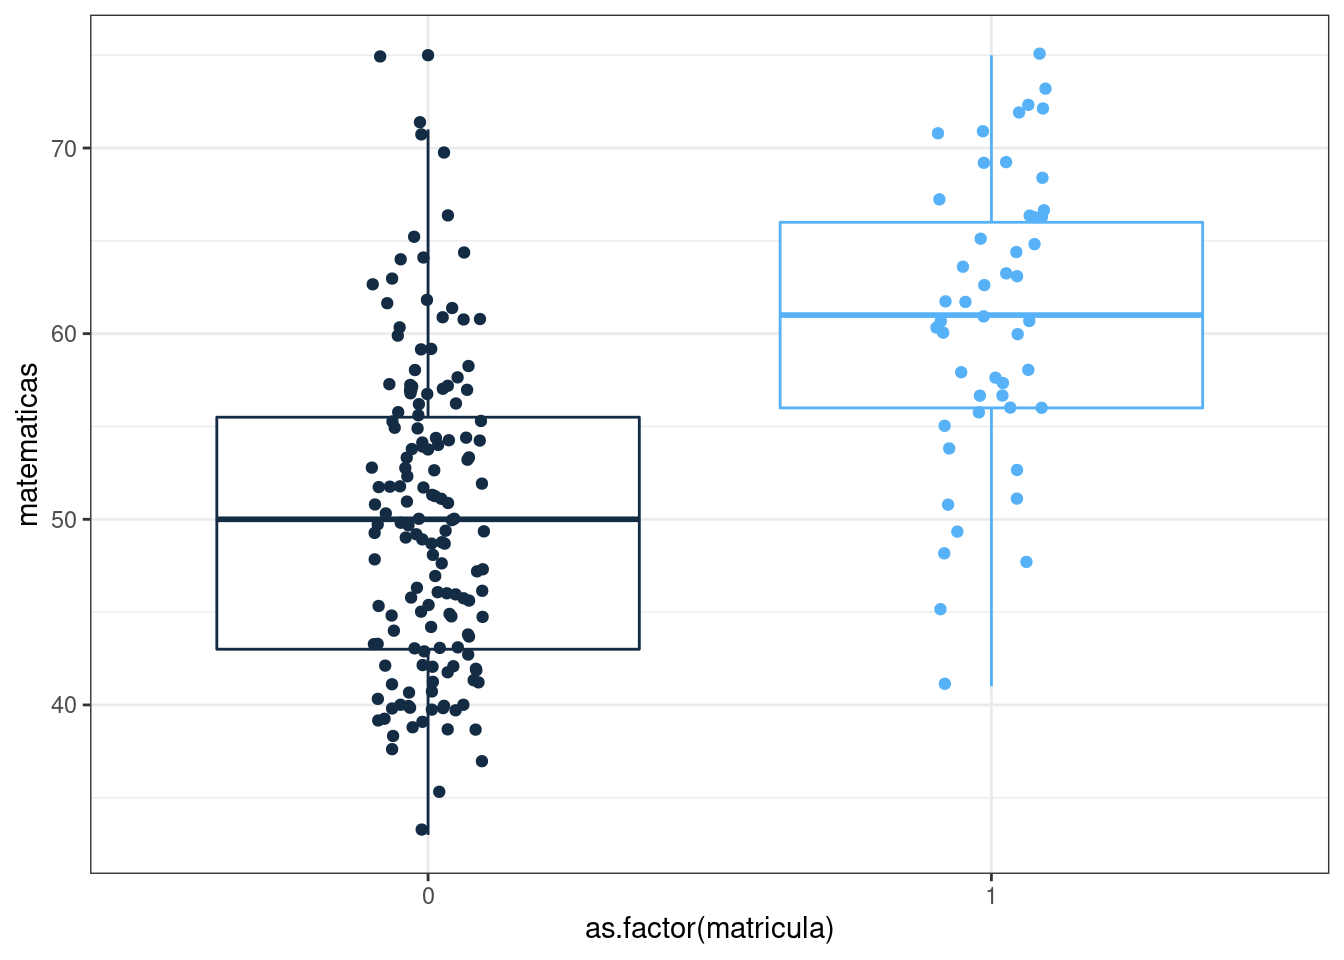
\includegraphics{logit1_files/figure-latex/unnamed-chunk-3-1.pdf}

\hypertarget{modelo-logit}{%
\subsection{Modelo logit}\label{modelo-logit}}

Inicialmente podriamos explorar una estimación de MCO, como posibilidad
de estimación:

\begin{Shaded}
\begin{Highlighting}[]
\NormalTok{modelo0 }\OtherTok{=} \FunctionTok{lm}\NormalTok{(matricula }\SpecialCharTok{\textasciitilde{}}\NormalTok{ matematicas)}
\FunctionTok{summary}\NormalTok{(modelo0)}
\end{Highlighting}
\end{Shaded}

\begin{verbatim}
Call:
lm(formula = matricula ~ matematicas)

Residuals:
     Min       1Q   Median       3Q      Max 
-0.76516 -0.27653 -0.06712  0.17720  1.02596 

Coefficients:
             Estimate Std. Error t value Pr(>|t|)    
(Intercept) -0.979947   0.150883  -6.495 6.57e-10 ***
matematicas  0.023268   0.002822   8.245 2.25e-14 ***
---
Signif. codes:  0 '***' 0.001 '**' 0.01 '*' 0.05 '.' 0.1 ' ' 1

Residual standard error: 0.3729 on 198 degrees of freedom
Multiple R-squared:  0.2556,    Adjusted R-squared:  0.2518 
F-statistic: 67.99 on 1 and 198 DF,  p-value: 2.248e-14
\end{verbatim}

\begin{Shaded}
\begin{Highlighting}[]
\NormalTok{g3}\OtherTok{=}\FunctionTok{ggplot}\NormalTok{(}\AttributeTok{data =}\NormalTok{ datos, }\AttributeTok{mapping =} \FunctionTok{aes}\NormalTok{(}\AttributeTok{x=}\NormalTok{matematicas, }\AttributeTok{y=}\NormalTok{matricula)) }\SpecialCharTok{+} 
           \FunctionTok{geom\_point}\NormalTok{() }\SpecialCharTok{+} 
           \FunctionTok{theme\_bw}\NormalTok{() }\SpecialCharTok{+} 
           \FunctionTok{geom\_smooth}\NormalTok{(}\AttributeTok{method=}\StringTok{\textquotesingle{}lm\textquotesingle{}}\NormalTok{, }\AttributeTok{formula=}\NormalTok{y}\SpecialCharTok{\textasciitilde{}}\NormalTok{x, }\AttributeTok{se=}\ConstantTok{FALSE}\NormalTok{, }\AttributeTok{col=}\StringTok{\textquotesingle{}dodgerblue1\textquotesingle{}}\NormalTok{)}

\NormalTok{g3}
\end{Highlighting}
\end{Shaded}

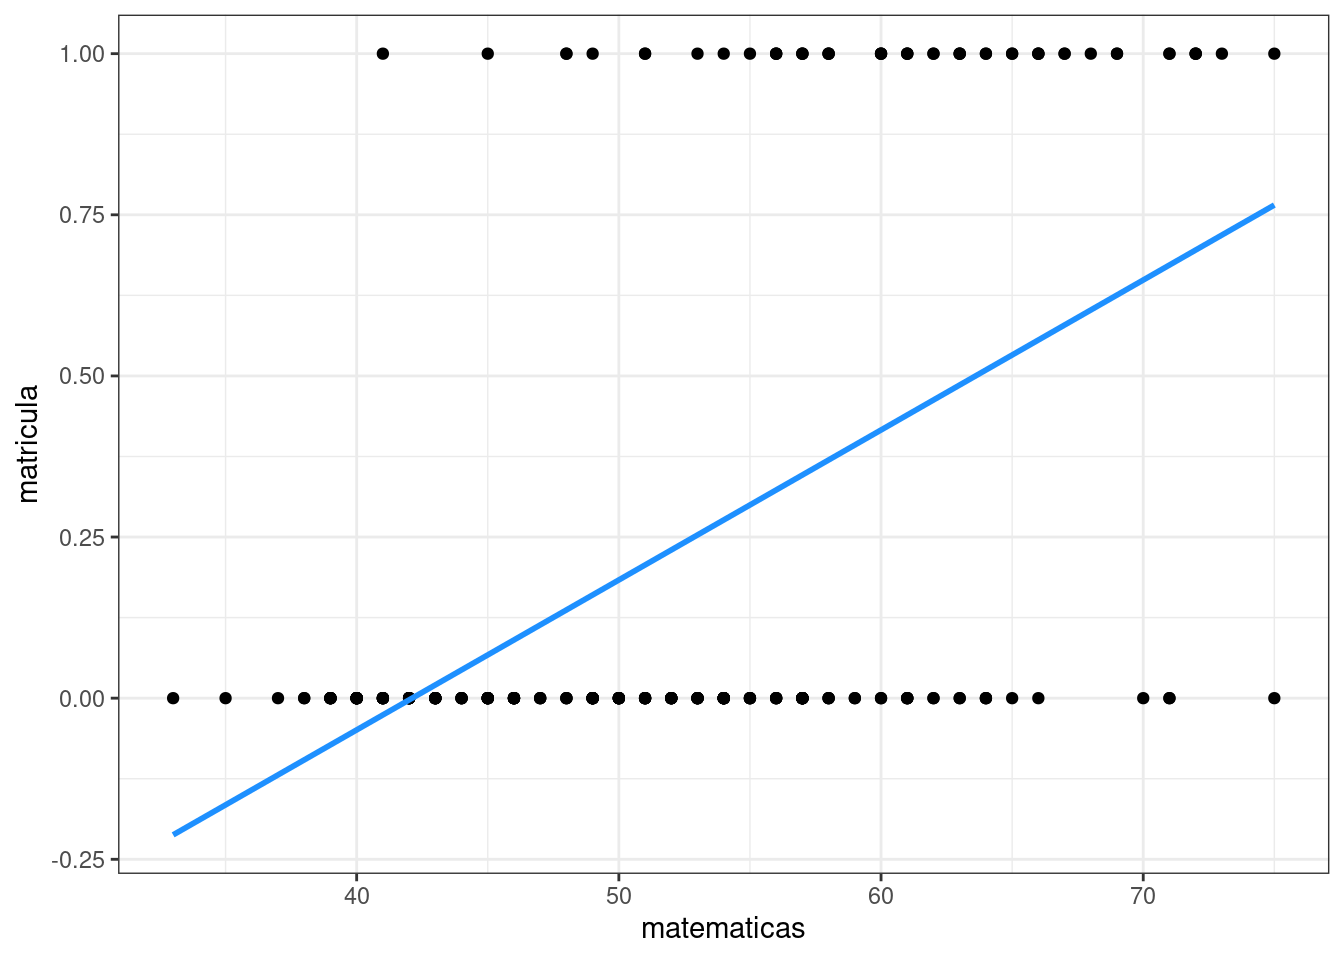
\includegraphics{logit1_files/figure-latex/unnamed-chunk-5-1.pdf}

Como se puede observar este modelo no permite ajustar una linea que
represente los valores obtenidos en la prueba de matematicas. Además de
no cumplir con los supuestos planteados para el modelo de regresión
lineal simple.

\begin{itemize}
\tightlist
\item
  No normalidad de los errores
\item
  Heteroscedasticidad de u
\item
  Posibilidad de que \(\widehat{Y_{i}}\) se encuentre por fuera del
  rango \([0,1]\), estimación de la probabilidad de \(Y\)
\item
  Valores muy bajos para \(R^{2}\), dada la dificultad de ajuste para
  una lina reacta
\end{itemize}

Estos problemas los podemos superar al plantear el siguiente modelo
teniendo como base la función de distribución acumulada \$F(x) = P(X
\leq x) \$ y la función logistica \(f(x)= \dfrac{1}{1+\exp{\{-x\}}}\)

\begin{Shaded}
\begin{Highlighting}[]
\NormalTok{fx}\OtherTok{=}\ControlFlowTok{function}\NormalTok{(x)\{}
   \DecValTok{1}\SpecialCharTok{/}\NormalTok{(}\DecValTok{1}\SpecialCharTok{+}\FunctionTok{exp}\NormalTok{(}\SpecialCharTok{{-}}\NormalTok{x))}
\NormalTok{\}}
\NormalTok{x}\OtherTok{=}\FunctionTok{seq}\NormalTok{(}\AttributeTok{from =}\SpecialCharTok{{-}}\DecValTok{10}\NormalTok{ ,}\AttributeTok{to=} \DecValTok{10}\NormalTok{, }\AttributeTok{by=} \FloatTok{0.1}\NormalTok{)}
\NormalTok{f}\OtherTok{=}\FunctionTok{fx}\NormalTok{(x)}
\FunctionTok{plot}\NormalTok{(x,f, }\AttributeTok{type=}\StringTok{"l"}\NormalTok{, }\AttributeTok{col=}\StringTok{"\#BC2B6A"}\NormalTok{, }\AttributeTok{lwd=}\DecValTok{5}\NormalTok{)}
\FunctionTok{grid}\NormalTok{()}
\end{Highlighting}
\end{Shaded}

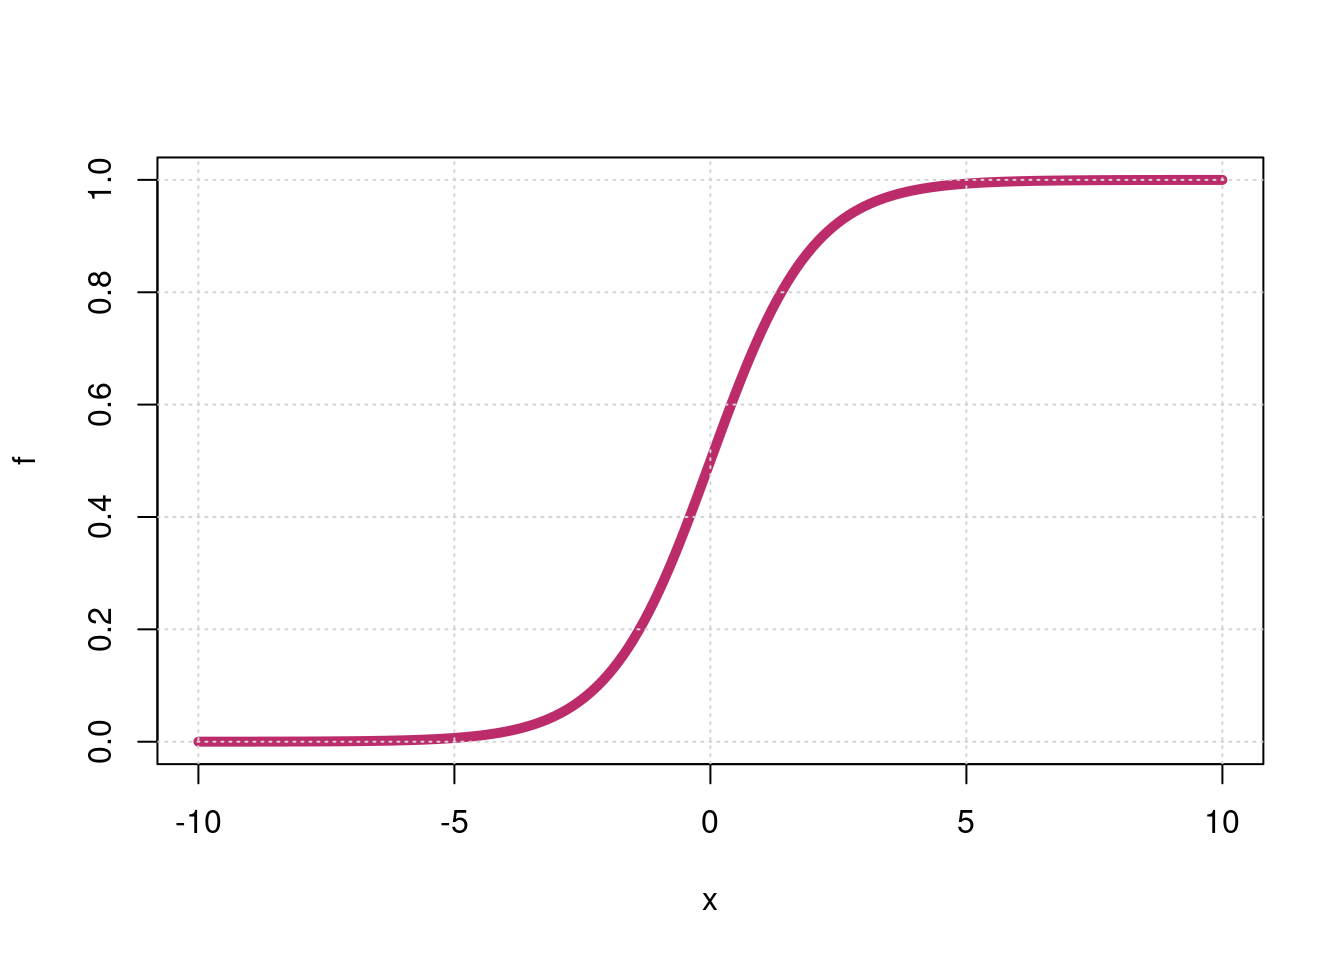
\includegraphics{logit1_files/figure-latex/unnamed-chunk-6-1.pdf}

Empleando la funcion logistica se replantea el modelo partiendo del
logaritmo de la razón de probabilidades en función de una combinación
lineal de las variables independientes :

\[\ln \Bigg(\dfrac{P(Y=k|X=x)}{1-P(Y=k|X=x)}\Bigg) =  \beta_{0}+ \beta_{1} \hspace{.2cm}x_{i} + u_{i}\]

Su estimación se puede plantear como:

\[\ln \Bigg(\dfrac{P_{i}}{1-P_{i}} \Bigg) = \ln (odds) =\beta_{0} + \beta_{1} \hspace{.2cm}x_{i} + u_{i}\]
Donde :

\begin{itemize}
\item
  \(odds = \dfrac{P_{i}}{1-P_{i}} = \dfrac{P(Y=k|X=x)}{1-P(Y=k|X=x)}\)
\item
  \(\ln(odds) = \ln \Bigg(\dfrac{P_{i}}{1-P_{i}} \Bigg) = \ln \Bigg(\dfrac{P(Y=k|X=x)}{1-P(Y=k|X=x)}\Bigg)\)
\item
  \(\ln \Bigg(\dfrac{1}{0}\Bigg) \hspace{.5cm}\text{si el estudiante RECIBE matricula de honor}\)
\item
  \(\ln \Bigg(\dfrac{0}{1}\Bigg) \hspace{.5cm}\text{si el estudiante NO RECIBE matricula de honor}\)
\item
  Si \(p = 1-p\) entonces \(odds = 1\) , por tanto \(\ln(odds) = 0\)
\item
  Si \(p < 1-p\) entonces \(odds < 1\) , por tanto \(\ln(odds) < 0\)
\item
  Si \(p > 1-p\) entonces \(odds > 1\) , por tanto \(\ln(odds) > 0\)
\end{itemize}

Para realizar la estimación del modelo logit utilizamos la función
\texttt{glm}

\begin{Shaded}
\begin{Highlighting}[]
\NormalTok{modelo1 }\OtherTok{\textless{}{-}} \FunctionTok{glm}\NormalTok{(matricula }\SpecialCharTok{\textasciitilde{}}\NormalTok{ matematicas, }\AttributeTok{data =}\NormalTok{ datos, }\AttributeTok{family =} \StringTok{"binomial"}\NormalTok{)}
\FunctionTok{summary}\NormalTok{(modelo1)}
\end{Highlighting}
\end{Shaded}

\begin{verbatim}
Call:
glm(formula = matricula ~ matematicas, family = "binomial", data = datos)

Deviance Residuals: 
    Min       1Q   Median       3Q      Max  
-2.0332  -0.6785  -0.3506  -0.1565   2.6143  

Coefficients:
            Estimate Std. Error z value Pr(>|z|)    
(Intercept) -9.79394    1.48174  -6.610 3.85e-11 ***
matematicas  0.15634    0.02561   6.105 1.03e-09 ***
---
Signif. codes:  0 '***' 0.001 '**' 0.01 '*' 0.05 '.' 0.1 ' ' 1

(Dispersion parameter for binomial family taken to be 1)

    Null deviance: 222.71  on 199  degrees of freedom
Residual deviance: 167.07  on 198  degrees of freedom
AIC: 171.07

Number of Fisher Scoring iterations: 5
\end{verbatim}

El modelo estimado en su forma original :

\[\ln \Bigg( \dfrac{\widehat{P_{i}}}{1-\widehat{P_{i}}} \Bigg) = \widehat{\beta_{0}} + \widehat{\beta_{1}} \hspace{.2cm}x_{i}\]
Utilizamos la función inversa del logaritmo

\[\Bigg( \dfrac{\widehat{P_{i}}}{1-\widehat{P_{i}}} \Bigg) = \exp{\bigg\{ \widehat{\beta_{0}} + \widehat{\beta_{1}} \hspace{.2cm} x_{i}}\bigg\}\]
\[\Bigg( \dfrac{\widehat{P_{i}}}{1-\widehat{P_{i}}} \Bigg) = \exp{\big\{ -9.793942  + 0.1563404 \hspace{.2cm}x_{i}}\big\}\]
El coeficiente estimado \(\widehat{\beta_{0}}\) corresponde al valor
esperado del logaritmo de la razon de probabilidades
(\(\ln \Bigg(\dfrac{P_{i}}{(1-P_{i})}\Bigg)\) para un estudiante con
nota cero en matemáticas. Para leerlo enterminos de probabilidad
realizamos la siguiente transformación:

\begin{Shaded}
\begin{Highlighting}[]
\CommentTok{\# coeficientes estimados}
\NormalTok{b}\OtherTok{=}\NormalTok{modelo1}\SpecialCharTok{$}\NormalTok{coefficients}
\NormalTok{b0}\OtherTok{=}\NormalTok{b[}\DecValTok{1}\NormalTok{]; }\FunctionTok{names}\NormalTok{(b0)}\OtherTok{=} \StringTok{" "}
\NormalTok{b1}\OtherTok{=}\NormalTok{b[}\DecValTok{2}\NormalTok{]; }\FunctionTok{names}\NormalTok{(b1)}\OtherTok{=} \StringTok{" "}
\CommentTok{\#{-}{-}{-}{-}{-}{-}{-}{-}{-}{-}{-}{-}{-}{-}{-}{-}{-}{-}{-}{-}{-}{-}{-}{-}{-}}
\NormalTok{x}\OtherTok{=}\DecValTok{0}
\FunctionTok{exp}\NormalTok{(b0}\SpecialCharTok{+}\NormalTok{b1}\SpecialCharTok{*}\NormalTok{x)}
\end{Highlighting}
\end{Shaded}

\begin{verbatim}
             
5.578854e-05 
\end{verbatim}

\begin{Shaded}
\begin{Highlighting}[]
\FunctionTok{exp}\NormalTok{(b0}\SpecialCharTok{+}\NormalTok{b1}\SpecialCharTok{*}\NormalTok{x)}\SpecialCharTok{/}\NormalTok{(}\DecValTok{1}\SpecialCharTok{{-}}\FunctionTok{exp}\NormalTok{(b0}\SpecialCharTok{+}\NormalTok{b1}\SpecialCharTok{*}\NormalTok{x))}
\end{Highlighting}
\end{Shaded}

\begin{verbatim}
             
5.579165e-05 
\end{verbatim}

Ahora para interpretar el aporte que genera un punto adicional en la
nota de matemáticas sobre la probabilidad realizamos el siguiente
cálculo:

\[\exp{\{ 0.1563404 \}} = 1.169224\]

\begin{verbatim}
exp(0.1563404) =  1.169224
\end{verbatim}

Este valor representa un aumento de 0.01169224 sobre la probabilidad de
obtenre matricula de honor por el incremento de un punto adicional en la
nota de matemáticas

\hypertarget{interpretaciuxf3n-de-widehatbeta_0}{%
\paragraph{\texorpdfstring{Interpretación de
\(\widehat{\beta_{0}}\)}{Interpretación de \textbackslash widehat\{\textbackslash beta\_\{0\}\}}}\label{interpretaciuxf3n-de-widehatbeta_0}}

Cuando \(x=0\) la probabilidad de obtener matricula es de \(0.00005\) \%

\(\widehat{\beta_{1}}\) indica el cambio en \(ln(p/(1-p))\) debido a un
increento unitario en \(x\), por lo que es necesario sacar la funcion
inversa al logaritmo que es la función exponencial

Por cada unidad de aumento de \(x\) los \(odds\) de obtener matricula se
incrementan en : \(1.17\) veces

\begin{Shaded}
\begin{Highlighting}[]
\FunctionTok{exp}\NormalTok{(b1)}
\end{Highlighting}
\end{Shaded}

\begin{verbatim}
         
1.169224 
\end{verbatim}

Un intervalo de confianza para los coeficientes se puede obtener
mediante :

\begin{Shaded}
\begin{Highlighting}[]
\FunctionTok{library}\NormalTok{(MASS)}
\FunctionTok{confint}\NormalTok{(}\AttributeTok{object =}\NormalTok{ modelo1, }\AttributeTok{level =} \FloatTok{0.95}\NormalTok{ )}
\end{Highlighting}
\end{Shaded}

\begin{verbatim}
                  2.5 %     97.5 %
(Intercept) -12.9375208 -7.0938806
matematicas   0.1093783  0.2103937
\end{verbatim}

\begin{Shaded}
\begin{Highlighting}[]
\CommentTok{\# MEDIANTE BASE GRAPHICS SIN INTERVALOS DE CONFIANZA}
\CommentTok{\# Codificación 0,1 de la variable respuesta}
\NormalTok{datos}\SpecialCharTok{$}\NormalTok{matricula }\OtherTok{\textless{}{-}} \FunctionTok{as.character}\NormalTok{(matricula)}
\NormalTok{datos}\SpecialCharTok{$}\NormalTok{matematicas }\OtherTok{\textless{}{-}} \FunctionTok{as.numeric}\NormalTok{(matematicas)}

\FunctionTok{plot}\NormalTok{(matricula }\SpecialCharTok{\textasciitilde{}}\NormalTok{ matematicas, datos, }\AttributeTok{col =} \StringTok{"darkblue"}\NormalTok{,}
     \AttributeTok{main =} \StringTok{"Modelo regresión logística"}\NormalTok{,}
     \AttributeTok{ylab =} \StringTok{"P(matrícula=1|matemáticas)"}\NormalTok{,}
     \AttributeTok{xlab =} \StringTok{"matemáticas"}\NormalTok{, }\AttributeTok{pch =} \StringTok{"I"}\NormalTok{)}

\CommentTok{\# type = "response" devuelve las predicciones en forma de probabilidad en lugar de en log\_ODDs}
\FunctionTok{curve}\NormalTok{(}\FunctionTok{predict}\NormalTok{(modelo1, }\FunctionTok{data.frame}\NormalTok{(}\AttributeTok{matematicas =}\NormalTok{ x), }\AttributeTok{type =} \StringTok{"response"}\NormalTok{),}
      \AttributeTok{col =} \StringTok{"\#447270"}\NormalTok{, }\AttributeTok{lwd =} \DecValTok{3}\NormalTok{, }\AttributeTok{add =} \ConstantTok{TRUE}\NormalTok{)}
\FunctionTok{abline}\NormalTok{(}\AttributeTok{h=}\NormalTok{.}\DecValTok{50}\NormalTok{, }\AttributeTok{col=}\StringTok{"red"}\NormalTok{)}


\FunctionTok{grid}\NormalTok{()}
\end{Highlighting}
\end{Shaded}

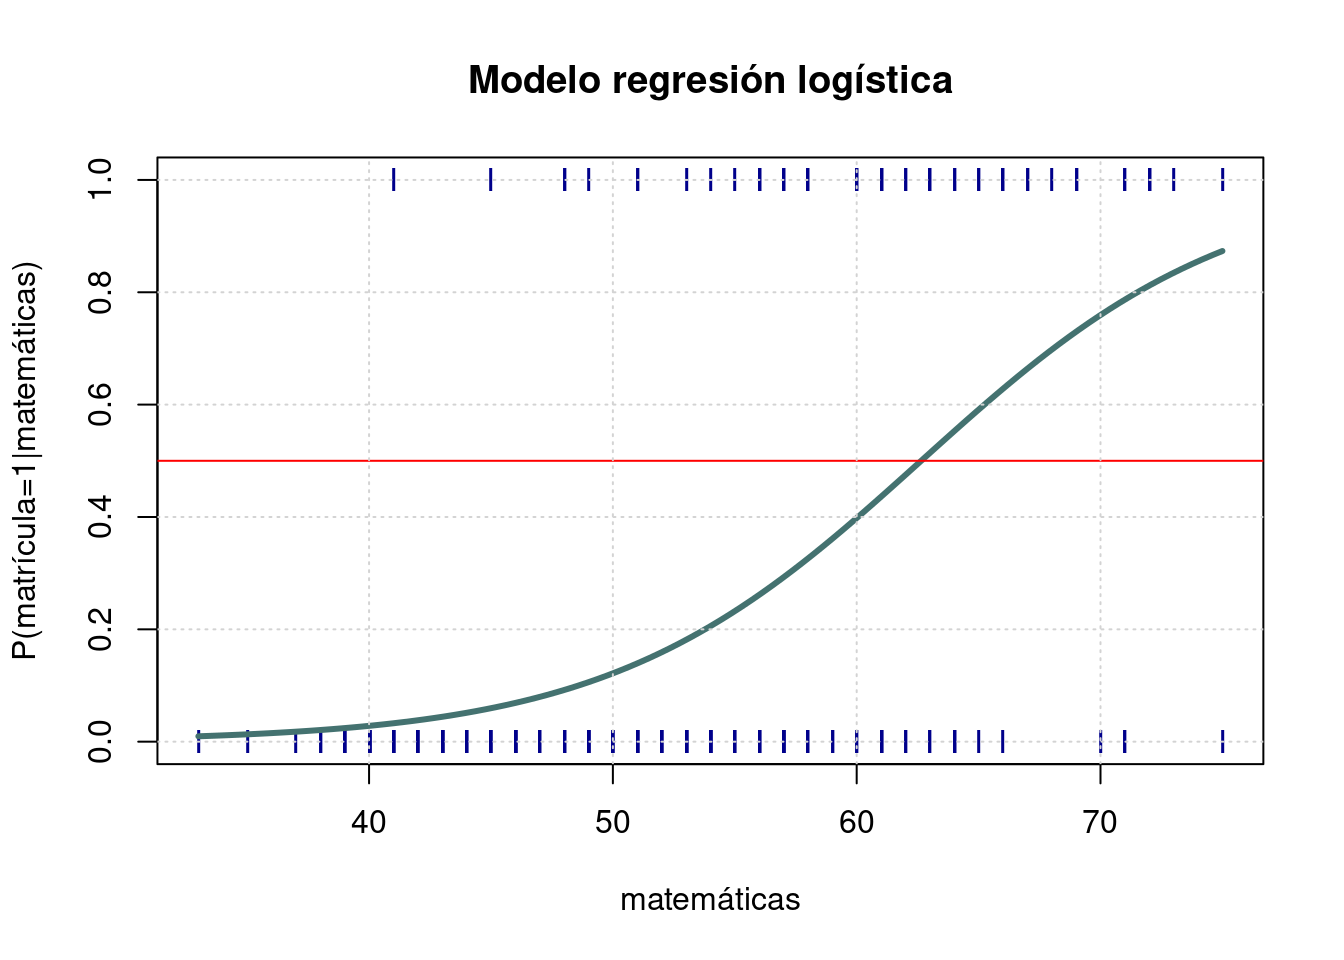
\includegraphics{logit1_files/figure-latex/unnamed-chunk-13-1.pdf}

\begin{Shaded}
\begin{Highlighting}[]
\FunctionTok{library}\NormalTok{(vcd)}
\NormalTok{predicciones }\OtherTok{\textless{}{-}} \FunctionTok{ifelse}\NormalTok{(}\AttributeTok{test =}\NormalTok{ modelo1}\SpecialCharTok{$}\NormalTok{fitted.values }\SpecialCharTok{\textgreater{}} \FloatTok{0.5}\NormalTok{, }\AttributeTok{yes =} \DecValTok{1}\NormalTok{, }\AttributeTok{no =} \DecValTok{0}\NormalTok{)}
\NormalTok{mc }\OtherTok{\textless{}{-}} \FunctionTok{table}\NormalTok{(modelo1}\SpecialCharTok{$}\NormalTok{model}\SpecialCharTok{$}\NormalTok{matricula, predicciones,}
                          \AttributeTok{dnn =} \FunctionTok{c}\NormalTok{(}\StringTok{"observaciones"}\NormalTok{, }\StringTok{"predicciones"}\NormalTok{))}
\NormalTok{mc}
\end{Highlighting}
\end{Shaded}

\begin{verbatim}
             predicciones
observaciones   0   1
            0 140  11
            1  27  22
\end{verbatim}

\begin{Shaded}
\begin{Highlighting}[]
\FunctionTok{mosaic}\NormalTok{(mc, }\AttributeTok{shade =}\NormalTok{ T, }\AttributeTok{colorize =}\NormalTok{ T,}
       \AttributeTok{gp =} \FunctionTok{gpar}\NormalTok{(}\AttributeTok{fill =} \FunctionTok{matrix}\NormalTok{(}\FunctionTok{c}\NormalTok{(}\StringTok{"\#447270"}\NormalTok{, }\StringTok{"\#f6b915"}\NormalTok{, }\StringTok{"\#f6b915"}\NormalTok{,}\StringTok{"\#447270"}\NormalTok{), }\DecValTok{2}\NormalTok{, }\DecValTok{2}\NormalTok{)))}
\end{Highlighting}
\end{Shaded}

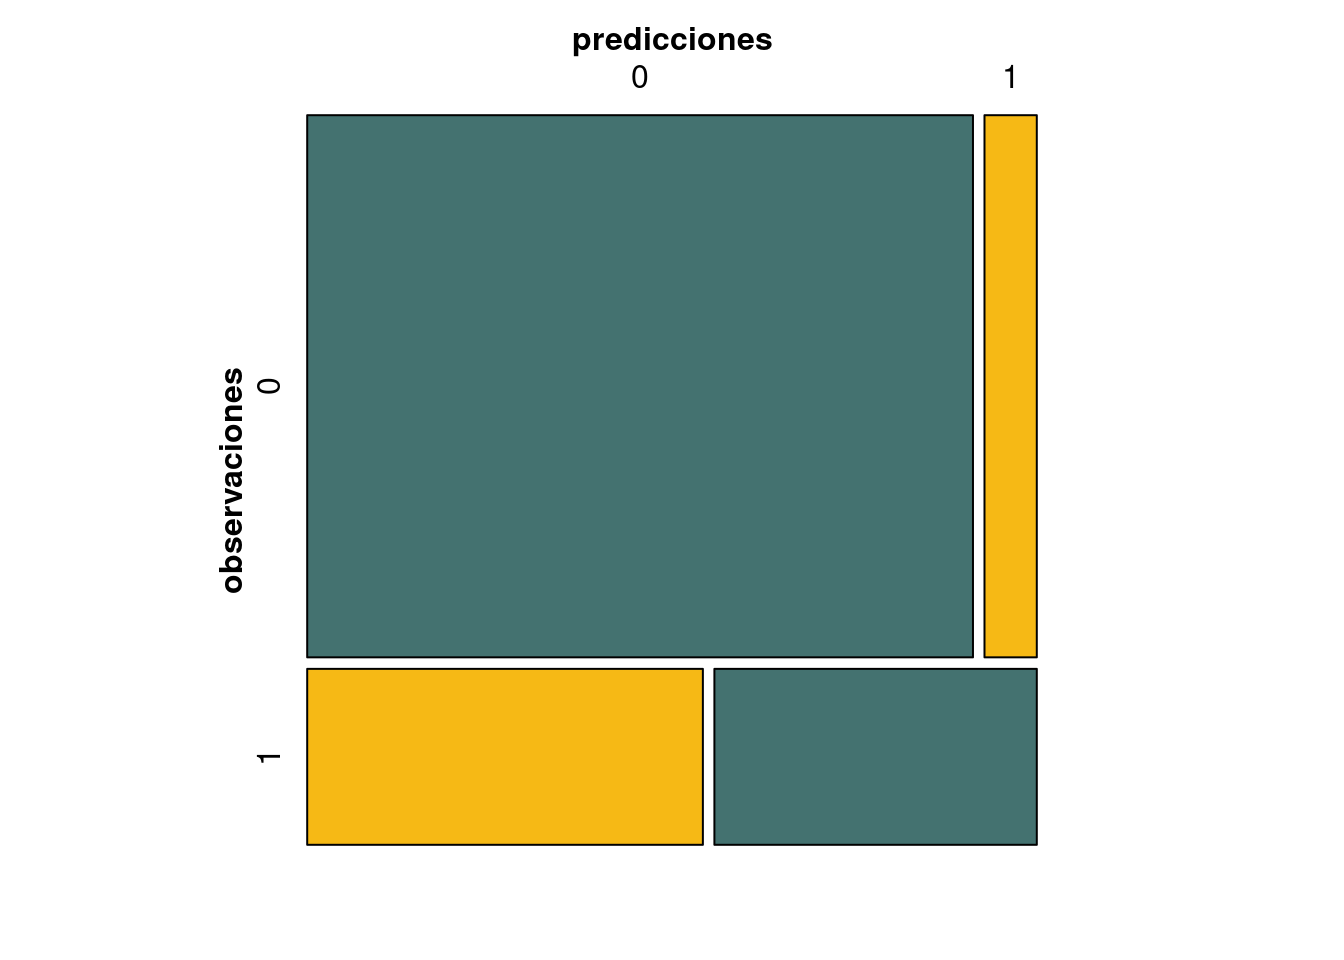
\includegraphics{logit1_files/figure-latex/unnamed-chunk-15-1.pdf}

Cuenta \(R^{2}\)

\begin{Shaded}
\begin{Highlighting}[]
\NormalTok{cuenta\_R2}\OtherTok{=} \FunctionTok{sum}\NormalTok{(}\FunctionTok{diag}\NormalTok{(mc))}\SpecialCharTok{/}\FunctionTok{sum}\NormalTok{(mc)}
\NormalTok{cuenta\_R2}
\end{Highlighting}
\end{Shaded}

\begin{verbatim}
[1] 0.81
\end{verbatim}

\begin{Shaded}
\begin{Highlighting}[]
\FunctionTok{library}\NormalTok{(DescTools)}
\FunctionTok{PseudoR2}\NormalTok{(modelo1, }\AttributeTok{which =} \StringTok{"McFadden"}\NormalTok{)}
\end{Highlighting}
\end{Shaded}

\begin{verbatim}
 McFadden 
0.2498172 
\end{verbatim}

\begin{Shaded}
\begin{Highlighting}[]
\FunctionTok{library}\NormalTok{(pscl)}
\FunctionTok{pR2}\NormalTok{(modelo1)}
\end{Highlighting}
\end{Shaded}

\begin{verbatim}
fitting null model for pseudo-r2
\end{verbatim}

\begin{verbatim}
         llh      llhNull           G2     McFadden         r2ML         r2CU 
 -83.5366186 -111.3550233   55.6368095    0.2498172    0.2428425    0.3615832 
\end{verbatim}

Predecir la probabilidad de que un estudiante pueda tener matricuala de
honor con un puntaje en matemáticas de 70 puntos

\begin{Shaded}
\begin{Highlighting}[]
\NormalTok{newdata1 }\OtherTok{\textless{}{-}} \FunctionTok{data.frame}\NormalTok{(}\AttributeTok{matematicas=}\FunctionTok{c}\NormalTok{(}\DecValTok{30}\NormalTok{,}\DecValTok{40}\NormalTok{,}\DecValTok{50}\NormalTok{,}\DecValTok{60}\NormalTok{,}\DecValTok{70}\NormalTok{))}
\NormalTok{newdata1}\SpecialCharTok{$}\NormalTok{rankP }\OtherTok{\textless{}{-}} \FunctionTok{predict}\NormalTok{(modelo1, }\AttributeTok{newdata =}\NormalTok{ newdata1, }\AttributeTok{type =} \StringTok{"response"}\NormalTok{)}
\NormalTok{newdata1}
\end{Highlighting}
\end{Shaded}

\begin{verbatim}
  matematicas       rankP
1          30 0.006037368
2          40 0.028186305
3          50 0.121647088
4          60 0.398068206
5          70 0.759489505
\end{verbatim}

\end{document}
